\section{Implementation}

We implement \sword\ in DPDK and P4. The P4 prototype
supports steering (\S\ref{sec:steering}) in Clover at
100-Gbps line rate, but does not perform the connection
multiplexing necessary to enforce ordering
(\S\ref{sec:connection_multiplexing}) that our full-featured
DPDK implementation provides.

%all of the functionality described
%previously; the P4 prototype does  but includes sufficient logic
%to perform conflict avoidance in
%for identifying and
%tracking connections, and resolving read and write conflicts in
%Clover.
%Connection multiplexing is implemented separately on a DPDK
%middlebox discussed further in this section.

\subsection{P4 implementation}

%\textbf{Switch Resource Utilization}
\begin{figure}[t]
    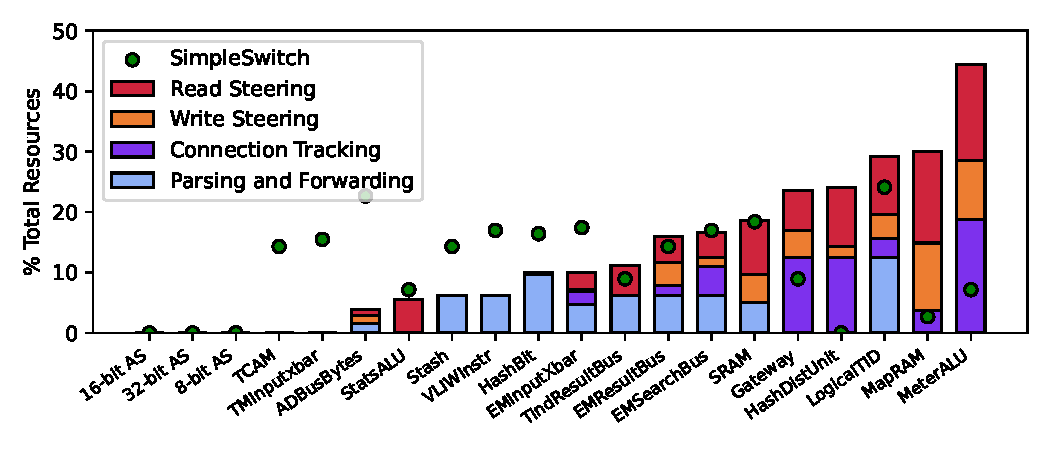
\includegraphics[width=0.485\textwidth]{fig/switch_resources.pdf}
  \vskip -0.5em
    \caption{Breakdown of switch resource utilization by \sword\ component.}
    \label{fig:switch_resources}
      \vskip -1em
\end{figure}

Steering is straightforward to implement in P4. We use P4 registers to
store connection state, virtual addresses, and outstanding
requests. Switch registers are constrained to 32, 16 and 8-bit blocks,
and are bound to specific switch pipeline
stages~\cite{netcache}. Packets visit each stage exactly once, so
register reads and writes must be pipelined correctly so that the same
stage which stores a virtual address on a write, is the same that
produces the address for CAS and read. Because registers are fixed
width, some lookups take multiple stages.  We use two-stage lookups
for (64-bit) virtual addresses with two 32-bit registers, and a single
stage for queue pairs, sequence numbers, and connection IDs.
%\sword's
%switch resource utilization is detailed in
%Appendix~\ref{sec:appendix_resources}.
Prior work has demonstrated that RDMA ICRC's can be implemented in a
P4 switch, but are redundant with the Ethernet CRC
~\cite{p4telemetry,bedrock}.  Hence, like previous
authors~\cite{switchml}, we disable ICRC checks at sender and receiver
NICs and do not update them at the switch.


Figure~\ref{fig:switch_resources} provides a breakdown of
the resource consumption of our P4 \sword\ implementation as
reported by
%. We collected these values from our testbed using
the Barefoot SDE version 9.7.0. Each percentage is
the average value across the total 16 switch pipeline
stages. {\sword} fits into 8 stages, and is run entirely on
the ingress pipeline.
%Parsing and traffic identification are simple in P4.
We use the header parser from the P4 simple switch to parse up to the
UDP header and create our own header parser for RoCEv2 and Clover
headers.  {\sword} uses RoCEv2 header, write, and CAS payload
information to identify traffic for steering. When new Clover traffic is
identified the connection is added to the connection tracker.
%and a
%connection ID is generated.
%at rack scale.

% P4 is a highly constrained language. For example it does not support loops.
% Architecturally P4 switches are also highly constrained. Packet parsing must be
% performed using the limited TCAM resources available on the switch, conditionals
% have a limited branching factor (4). Packets are processed in stages, and device
% memory from one stage cannot be accessed at the next, therefore branching
% conditionals which access the same variables must be aligned to the same switch
% stage if they are to read or write to the same variables. In this section we
% describe our P4 implementation of {\sword} and how it adheres to the constraints
% of P4 and programmable switches.

% \textbf{Parsing} {\sword} has no special requirements for packet parsing. Our
% design is focused on RoCEv2 which runs over UDP. Our prototype implements
% Ethernet, IP, UDP and RoCEV2 parsing. RoCEv2 headers are required for reading,
% and manipulating virtual addresses. One additional header is required for Clover
% to read the key out of write requests.

% \textbf{Resource Utilization} {\sword} requires SRAM to cache data structure
% information. The amount of data required is dependent on the data structure
% itself. In clover we cache the last virtual address of each key, and we keep a
% cache 3x the size of the keyspace for read steering.


% \textbf{Traffic identification} Depending on the disaggregated
% rack architecture, memory traffic might be coresident with regular
% network traffic.  Additionally some of the traffic on the memory bus
% may not require tracking or manipulation. In the case of Clover we do
% not interpose upon or modify traffic to the metadata server as it is
% not in the read/write path. The first stage of our packet-processing
% pipeline classifies requests for manipulation. In our design operators
% submit a filter as part of their configuration to allow traffic which does
% not need to be modified to flow freely.

% \textbf{Dynamic connection tracking}
%  A key goal of our approach is to support
% serializer-based performance enhancements without modifying the far memory
% system itself---including requiring any explicit negotiation with the
% serializer.  We add and subtract RoCE connections to {\sword}'s management
% tables based upon the send and receipt of CAS operations. The QP and sequence
% number for the CAS are stored on send, and the ATOMIC ACK is used to obtain the
% other recever's QP.  As this approach requires only a single packet, requests
% can be added and removed from our algorithm dynamically with little effort.

%For instance is designed to deal with memory operations made to the wrong
%location via iterative pointer chasing. We strongly suggest that disaggregated
%algorithms take this approach as our middlebox solution only acts to acclerate
%operations in the common case.


% \textbf{Initializing connection mapping}
% \sg{dpdk only}
% As some state may be dependent on the number of connections (such as the
% key-to-QP and lock-to-QP mappings), state transitions either require a lock, or
% the copying of current state over to a new epoch when new connections are added.
% In all of our experiments only one such transition is made. We begin our mapping
% after a specific number of clients for the experiment have connected. Once the
% total number of clients have connected, a switch is flipped, and the QP
% multiplexing algorithm begins. Requests which do not have mappings stored, but
% were in flight during the flip have their sequence numbers and MSN values
% applied to the connection state of the new epoch.

%\subsection{Operation caching}
%\label{sec:operation-caching}



% \begin{figure}
%     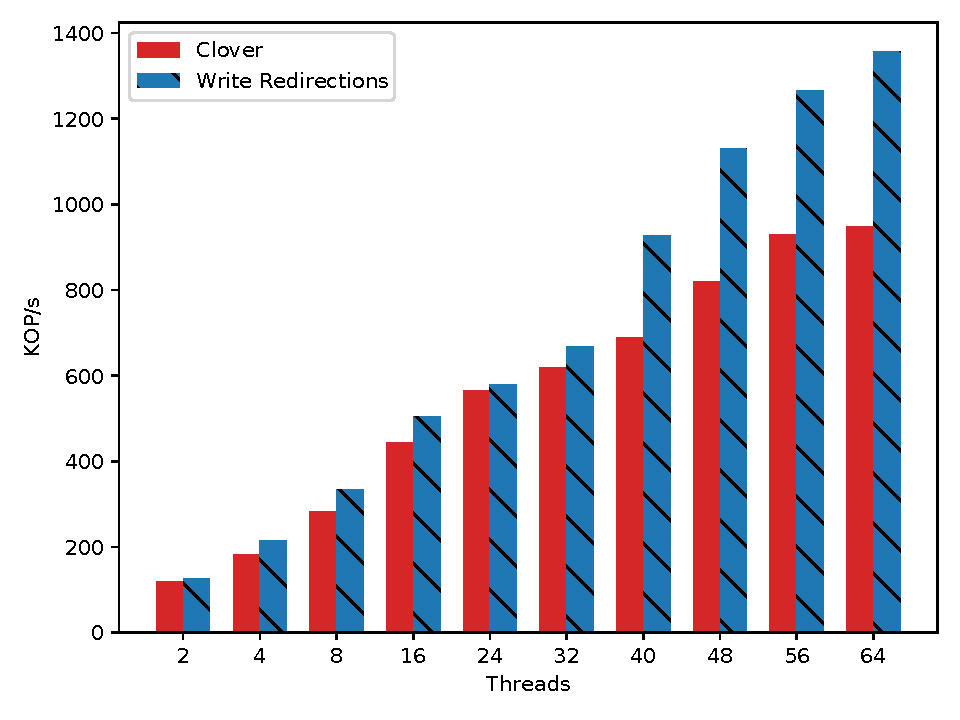
\includegraphics[width=0.45\textwidth]{fig/throughput.pdf}
%     \caption{Default Clover throughput vs. Clover with write conflict
%     detection and correction turned on \todo{recompute with the read caching values (old)}}
%     \label{fig:throughput}
%     \vskip -1em
% \end{figure}

% \subsection{Implementing Atomic replacement}

% In the
% following subsections we describe the dangers of removing atomics, and present
% our solutions.

% A few assumptions must be made in order for this replacement of operations to be
% made. First and foremost all operation serialization must be made, and finalized
% at the point where the CAS is swapped out. More formally, all of the data
% structure invariants which required locking, must be satisfied at the time of
% transforming the packet. Further the order of operations must be maintained
% downstream from the checking of the invariant. These two requirements influence
% the design of any system which aims to make this performance improvement.


%% ACS - This is just lifted from WORDS; no need to repeat here

%% \begin{figure}
%%     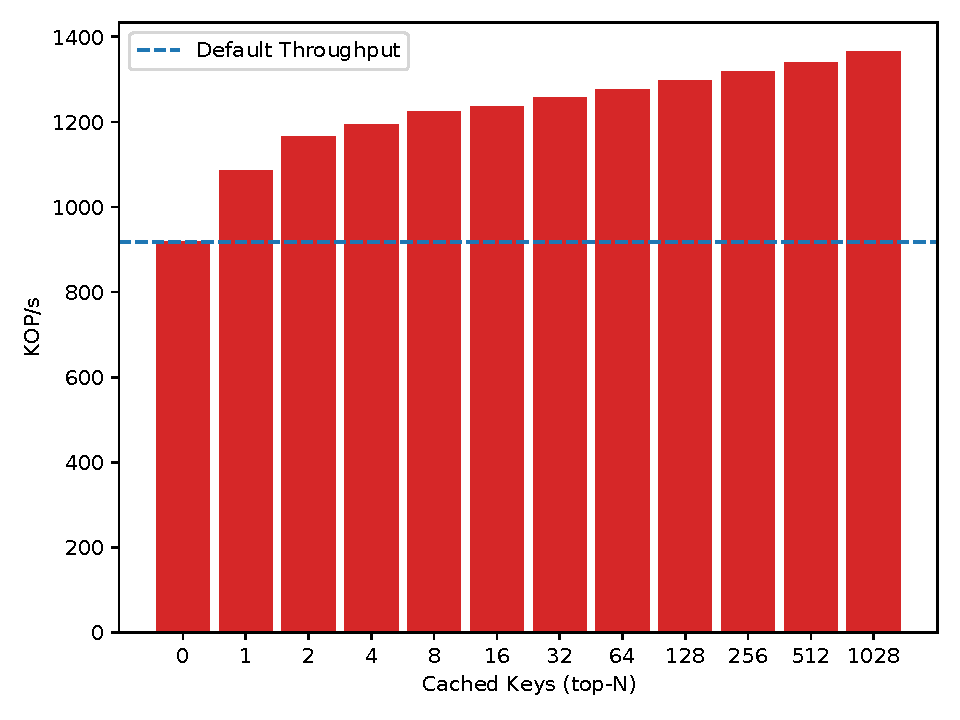
\includegraphics[width=0.45\textwidth]{fig/cache.pdf}
%%     \caption{Performance as a function of keys cached. Caching a few
%%     of the top-$N$ keys provides the greatest marginal throughput
%%     benefits.}
%%     \label{fig:cache}
%% \end{figure}

%% \textbf{reduced cache size} we show that if hot keys are known we require only a
%% small amount of in network state~\ref{fig:cache} we have considered dynamic
%% approaches such as LRU which would allows for a finite amount of space and an
%% arbitrary number of keys to be serviced.

% The first requirement, that the structural invariants
% of the data structure be maintained at the point of transformation demands that
% all of the state required to check the structural invariant be present at the
% point in the network at which the swap is made. This fact increases the memory
% cost on a switch, however with intelligent data structure design the cost of the
% required metadata can be mitigated. In the case of Clover, while each key has
% an entire linked list history that can potentially span megabytes, the only
% required metadata to make the change from CAS to write is the location of the
% tail pointer. In this case the metadata cost is O(n) as it grows linearly with
% the keyspace.

% \textbf{2) reordering} The second requirement, that operations not be reordered
% after the invariant has been checked requires more care in real systems. For
% instance in an RDMA system with two clients, both could have contesting CAS
% operations swapped with writes. As the two clients are transmitting operations on
% separate QP, and the receiving NIC makes no guarantees about ordering between QP,
% the operations could easily be reordered. In the case with CAS, the order could
% be forced by ensuring that if one write was to succeed the second would fail.
% Without this guarantee the preservation of operation ordering must be maintained
% in another way.

% \subsection{Connection Remapping}


% Our solution here is simple, given that we have the key's for reads and writes
% (Section ~\ref{sec:operation-caching}), all operations for the same key are
% mapped to the same QP.  This algorithm requires that a few pieces of state be
% maintained per connection.  First the sending and response QP for each sender
% and receiver need to be tracked. Second the sequence number of each connection,
% and the original message sequence number offset must be maintained. Per client
% connection the pair of QP's require 48 bits, and the sequence + message sequence
% require an additional 48 for a total of 12 bytes per connection. The storage
% requirement for mapped requests varies based on the algorithm. If clients are
% able to issue an unbounded number of async requests, then a buffer large enough
% to maintain backwards mappings for each request is required. In clover clients
% can issue up to 2 async requests, so we keep a two 6 byte mappings for each
% connection available to map back. 

% Depending on the algorithm and the QP mapping scheme requests from a single
% sender can be reordered. That is, if a client makes a read and write request to
% different locations in memory, and they are mapped to different QP, they may be
% returned out of order. Infiniband allows for out of order operations on
% receivers~\cite{infiniband-spec}, which pushes operation ordering to client
% side user space. Roce does not allow for out of order operations. In this case
% the receiving NIC will retransmit if requests are delivered out of order. Here
% we buffer requests in network, as we have application knowledge the size of the
% buffer is bounded (to the size of a single read packet in clovers case). We
% suggest that given the tight memory restrictions on middleboxes algorithms which
% have an unbounded number of async requests leave the ordering of remapped
% requests to client side user space using IB verbs or a different transport layer
% entirely.


% \subsection{DPDK considerations}

% {\sword} is implemented in DPDK for ease of programmability, but
% requires that all requests are processed without the aid of RDMA
% hardware on the NIC. Using DPDK introduces issues in terms of
% performance as individual cores on the server have low packet
% processing capabilities relative to dedicated networking hardware. As
% such our design is multithreaded and requires the use of careful
% atomics for performance.  Our design partitions cores into TX and RX
% groups. RX cores are configured via RSS and perform traffic
% identification, write steering and mapping. We completely removed the
% need for any explicit locking between cores and share as little state
% as is theoretically possible. Each TX core serializes requests by
% making atomic fetch-and-add updates to a shared region of memory
% containing connection sequence and message-sequence numbers. RX cores
% are handed packets from TX cores using DPDKs lock-less ring
% library. TX cores check packets to determine if they require CRC
% computation and calculate the CRC only if the packet has been
% modified. Adding a packet handoff between TX and RX increases latency,
% however the head-of-line blocking incurred by having a single core
% perform both mapping and CRC calculations is too high for our purposes.

% We find that by using an array size of
% 3$\times$ the vast majority of reads succeed first try.
% For
% performance reasons we forgo heavyweight hash functions and use
% the \texttt{murmur3} bit scrambler to attain an approximately even
% hash of virtual addresses in only a few cycles.

%\paragraph{Switch resources}
%\label{sec:appendix_resources}
%


\subsection{DPDK vs P4}

\begin{figure}
  \center
    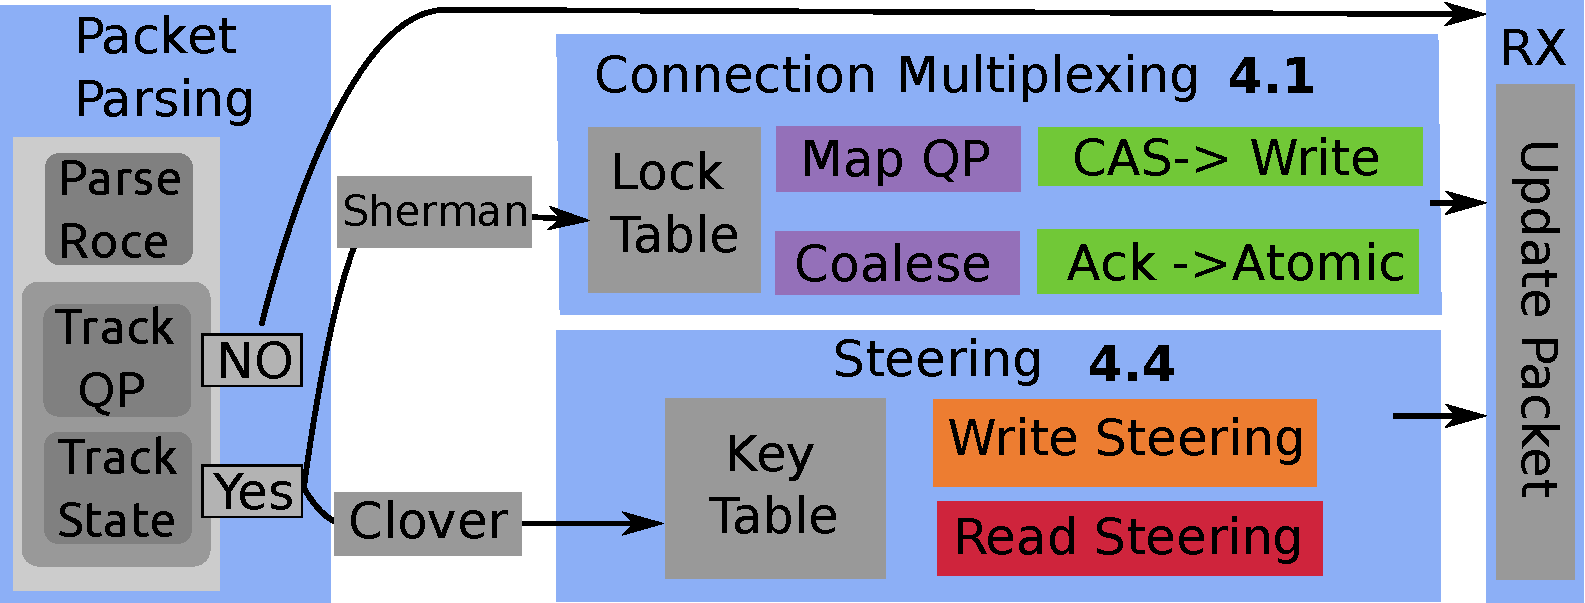
\includegraphics[width=0.45\textwidth]{fig/swordbox_overview.pdf}
    \caption{\sword's DPDK processing pipeline.}
    \label{fig:system}
  \vskip -1em
\end{figure}

Our P4 prototype does not currently support connection
multiplexing due to hardware limitations of our switch and
RDMA NICs. Our DPDK \sword\ implementation (shown in
Figure~\ref{fig:system}) consists of 3,392 lines of C and
includes all of the features described in the previous
section---including ICRC recalculation.
%(see Appendix~\ref{sec:appendix_icrc}).
In this section we describe why tracking outstanding
requests and de-coalescing ACKs is challenging in current
RMT hardware, and suggest small hardware modifications which
would make a P4 implementation simpler.


\textbf{Connection mapping.} Each memory bound RDMA packet
generates a map entry to demultiplex responses back to its
original connection. On incast (all clients sending to the
same resource) a connection must have enough preallocated
mapped entries in its ring buffer for every connected
client. 
%%
Because switch registers are allocated at compile time,
statically provisioning for the worst case requires $O(n^2)$
space complexity ($n$ entries for every connection).
Supporting only 512 clients requires 2MB of SRAM (1/16th of
a Tofino's total buffer space) given this constraint.
Storing these 64-bit entries takes 2 pipeline stages in the
best case, and 8 in the worst (8-bit registers).

%In the worst number of in flight requests with $n$ close
%looped clients is $n$, so $n^2$ is dramatic over
%provisioning. However, s
Space-efficient alternatives are harder to implement. Hash
tables have much better space utilization, but collisions
are hard to deal with. For each potential collision,
additional pipeline stages must be allocated and entries
must include QP IDs to check for collisions---increasing a
single hash table lookup to four stages.
%, which is multiplied for each potential collision.
At millions of packets per second collisions are common (3
or more) which exceeds the pipeline length of Tofino
switches.

%\textbf{(Fix) Dynamic Memory Allocation:} 
%%
%If registers could be resized at runtime, or dynamically mapped with
%a virtual we could resize our entry tables at runtime and steal from
%space from under utilized connections. This has the potential to
%decrease our memory utilization to clost to $O(n)$. This is a trivial
%task with an allocator and pointers, but a prohibitively hard task
%with static registers and single stage lookups.



% \textbf{Connection Mapping:} Connection mapping requires the storage of a 64 bit
% mapping entry for each in flight request (old\_seq, new\_seq, conn\_id,
% cas\_to\_write, opcode). These map entries are space concern on programmable
% switches. Mapped entries are stored per connection. When an request is mapped to
% a connection the entry is generated, when a response returns the entry is
% removed.In the worst case, any connection may need to store outstanding requests
% for the total number of connected clients as each client could asynchronously
% issue a request for the same lock concurrently. 

% We use connection sequence numbers to look up requests as they are unique for
% each connection, have no collisions, and only require an offset for lookup
% ($sequence\_number \% max\_clients$). The programmable switch requires that all
% storage be allocated at compile time, so we need to provision for the worst case
% scenario.  The space requirement grows $O(n^2)$ with the number of clients as
% each connection must be statically allocated with enough space to handel a worst
% case burst.

% Given static allocation if we want to support 512 client threads (the order of
% our experiments), in the worst case we need 1024 * 1024 * 8 bytes of connection
% storage. 8MB is not much storage, but on our Tofino switch this represents 1/4
% of the total SRAM assuming the compiler packs requests perfectly. Unfortunately
% this is unlikely the case.  Making this mater worse is that much of switch
% memory is allocated into 8 and 16 bit registers. Only a few are allocated to
% read and write 32 bits. 2 pipeline stages are the minimum for connection
% remapping storage. In the worst case (using 8 bit registers) 8 are required (an
% entire pipeline). While expensive this is not a prohibitive cost to
% implementation.

% We could use a hash table shared by all connections as a lookup for mapping
% entries using the key $concat(qp\_id,sequence\_number)$ which would conceptually
% reduce the space complexity. However if a collision occurs the collision lookup
% must be done in a following stage of the pipeline. This increases the space cost
% by the size of the longest collision chain. It also increases the size of each
% entry from 64 to 88 as the original queue pair id must be stored alongside the
% map entry to detect collisions. This requiring 3 stages to store. Detecting a
% collision requires an additional stage to run a conditional statement on the
% queue pair id. A chain of 2 collisions therefore would require 8 stages -- our
% entire egress pipeline to resolve. Given that we are processing millions of
% packets per second on a maximum sized hash table of 16k entries, collisions of 3
% or more are common.


\textbf{Request coalescing.}
%As an optimization RDMA NICs
%frequently summarize multiple ACKs into a single ACK.
%Multiplexed connections must have each coalesced request
%reconstructed to prevent timeouts and retransmissions.
% In order to perform QP mapping, these ACKs must be
% iteratively reconstructed if the original requests were
% generated by different clients.  %
Transforming coalesced ACKs in P4 is extremely
challenging. A variable number---up to the number of
clients---of entries must be matched against every packet.
Yet, each stage of a P4 pipeline holds unique data and
supports only a single lookup.
%of the specified register size (8,16,32), as such we are
%unable to look up a variable number of requests to
%generated coalesced ACKs.
Replicating entries across stages would allow for multiple
lookups per packet but a server can coalesce
%. However as mentioned above map entires consume 2MB of
%SRAM. Further,
an arbitrary number of ACKs so no fixed number of
duplications suffice (and we frequently observe coalescing
of 10 or more requests).  Recirculation is another
alternative, but inflates bandwidth usage in the common case
and causes responses to be delivered in reverse order. 
%%
Disabling ACK coalescing at the server NIC would dramatically reduce
the complexity required to multiplex connections, but we are unaware
of a way to do so on Mellanox NICs.
% Of
% course, the issue could be avoided entirely if it were
% possible to disable coalescing on server NICs.
%We are not aware of a way to do so on ConnectX-5s.

% The most complex part of connection remapping is
% calculating coalesced ACKs. The fix for this is simple: Turn off ACK coalescing
% on the NIC, as it is only a performance optimization. This fix alone would allow
% our design to fit onto a Tofino chip.

% One option would have been to duplicate data, so that if a coalesce did occur,
% it could be detected by reading duplicate data in the next stage.  The
% difficulty is that under aggressive contention the coalescing 10 or more ACKS is
% a common occurrence and duplicate stages would be required for each coalesced
% response. Given that a 64 bit entry requires two stages duplicating is not an
% option as it would easily exhaust all pipeline stages and never guarantee
% correctness.

% Because of P4's fixed location registers and pipelines performing these lookups is hard.
% In dpdk this search and packet generation implemented in a 3 line function with
% a for loop. In P4 it this functionality was prohibitively difficult to engineer.
% The complexity is caused by the need to both search multiple entries of the
% outstanding connection list which is not supported by P4 table lookups. 

% Our greatest unmet challenge with connection mapping
% in P4 dealing with RDMA coalescing. When a response is mapped back to a client
% it may be a coalesced response, if so the prior map entry must be checked and an
% ack generated for that entry. This is an iterative process as a single response
% can have coalesced many other responses.

% \sg{I don't actually know if the following would work, it's an educated guess:}
% Another option is to use packet recirculation. We could duplicate data once, and
% perform a look back to the prior entry to determine if it was coalesce and then
% generate another packet to handle the handle the coalesced ack. 
% %%
% Performing this iteratively could generate all the required ACKs. However it
% dramatically increases complexity and inverts the order of packet delivery on
% the clients.

% \textbf{Conditional Complexity:} The final difficulty in implementing connection
% mapping in P4 are conditional statements. In P4 architectures branching is
% limited. At any conditional a max of 4 paths can exist.  In clover we reduced
% the total number of branching statements to 4 for each of the read, write, CAS,
% and ACK pathways. Connection remapping requires complex logic and arithmetic for
% generating message sequence numbers, storing request stubs across different
% register sizes, and detecting, and generating coalesced ACKs. Separately none
% of these issues are enough to prevent the implementation of connection remapping
% on a programmable switch. However in concert the P4 complier was not able to
% synthesize a program which could fit into our 16 stages of the Tofino 1. Future
% hardware such as Tofino 2 and 3 would likely be able to support this
% functionality due to having over double the pipeline logic.

% \subsubsection{Potential Fixes}

% \textbf{Complex Conditionals} Increasing the branching factor of conditionals
% would greatly decrease the complexity of implementing many complex protocol
% features. In some cases branching to 4 or more statements would have allowed
% lookups in the following stage to be implemented in a single stage rather than
% two.
